Despite a multitude of identified technical risks and ethical concerns, the authors of this paper claim that the emergence and development of the CA should not be simply avoided, but should rather be encouraged in such a manner that the moral autonomy of those who are willing to utilize the technology is respected while the possible risks are striven to be minimized. Moreover, we argue that an excessively conservative view which tries to indiscreetly restrict the entire human augmentation technology itself will not only hinder the gateway to the great benefits of the technology, but also limit the possibility to develop a more encompassing social, economical, technological, and ethical framework which would help us better comprehend the implications of the related technologies and allow us to deal with the risks more effectively.
%\vspace{-2.5cm}

As a way of utilizing the technology while minimizing the technical risks and ethical concerns, the authors propose the following recommendations:

%\vspace{-2.5cm}
\begin{itemize}
	\item Active encouragement of the application of CA technology for therapeutic purpose (e.g. prosthetic limbs for the amputees illustrated in Figure \ref{prosthetic_arm}, and visual prostheses for the blind illustrated in Figure \ref{prosthetic_eye}). Since such kind of use of the technology is much less controversial, it is recommendable that the development of the augmentation technology be focused on these medical fields for the time being. Once the technology gains more maturity and people become more familiar (and knowledgeable) with it, we can then have more meaningful discussions concerning the acceptability of the CA technology that is intended to enhance the human ability "beyond the normal level".
	\item Active encouragement of the development of non-permanent/wearable cybernetic devices, starting from the smallest scale. If the intrusive nature of the CA is removed, there will be much less technical risks and ethical concerns. Therefore, it can be a great stepping-stone for the introduction of the CA technology for similar reasons as in the previous item. 
	\item A discussion as to whether the CA is a key to Utopia or Dystopia can be meaningful as long as the discussion actively continues throughout the development and deployment of the technology, whilst refraining from making hasty conclusions (i.e. slippery slope fallacy). Note that CA is a very broad technology. Therefore, instead of judging the final possible outcome of the entire concept of the technology, one should rather try to find specific fields and aspects in which the technology can be applied with the highest acceptability. 
\end{itemize}

\begin{figure}[]
	\centering
		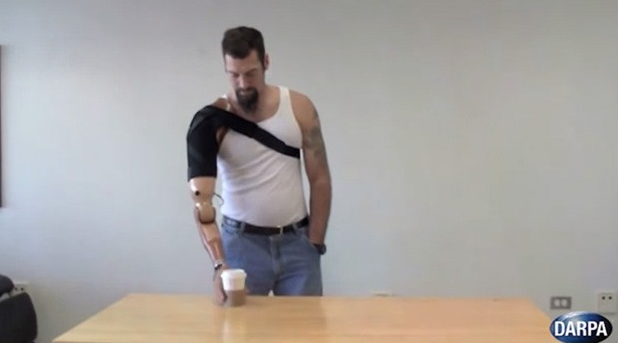
\includegraphics[width = 8cm]{prothesis_arm}
	\caption{Prosthetic arm developed by DARPA. An artificial arm is connected to the user's existing muscles and nerves\cite{prosthetic_arm}}
	\label{prosthetic_arm}
\end{figure}

\begin{figure}[]
	\centering
	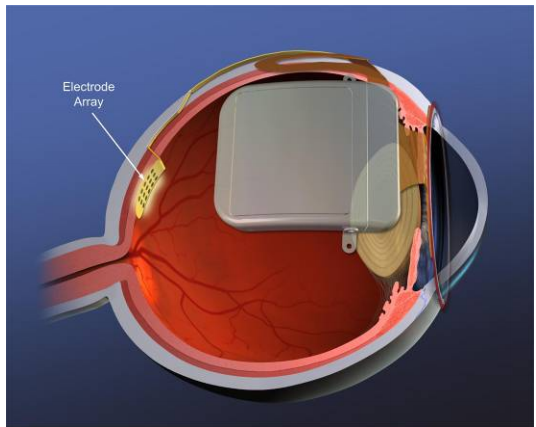
\includegraphics[width = 6cm]{prothesis_eye}
	\caption{Prosthetic retinal implant concept illustration \cite{retinal_implant}}
	\label{prosthetic_eye}
\end{figure}